\graphicspath{{09-Detector-alignment/Figures/}}

\section{Beam-based detector alignment}
\label{Sect:DA}

\subsection{Introduction}
\label{SubSect:DA_Intro}

To carry out its program, MICE requires all of its detectors to reconstruct space points in a globally consistent fashion. A beam-based alignment algorithm was developed to improve the resolution on the position of the scintillating-fibre trackers lodged inside the bores of superconducting magnets. This method can achieve unbiased measurements of the trackers rotation angles with a resolution of 6\,mrad/$\sqrt{N}$ and of their position with a resolution of 20\,mm/$\sqrt{N}$, with $N$ the number of selected tracks~\cite{2018arXiv1805.06623T}.

The single-particle nature of the MICE experiment requires reliable global track matching throughout, i.e. the ability to associate a trace measured in the upstream tracker with one in the downstream tracker but also with the particle identification detectors. The many detectors must reconstruct space points in a globally consistent fashion to guarantee reliable and efficient track matching, as well as unbiased muon scattering measurements.

The baseline for the beam-based alignment is the surveys of the detectors in the hall using laser telemetry, performed regularly throughout the commissioning and data taking, following any mechanical activity performed on the beam line and cooling channel. Only the trackers, nested in the superconducting solenoids, could not be accessed, so their position is inferred with respect to the flanges and the beam can be used to check the tracker stations alignment.

\subsection{Analysis method}
\label{SubSect:DA_Analysis}

The position of each tracker in global coordinates is entirely defined by the location of its centre and a set of three angles.
Since the coordinate of each tracker along the beamline is known to great accuracy from the survey and the rotation about $z$ has negligible influence on the alignment only 4 constants have to be find for each tracker.

The location of the TOFs is used as the reference for the tracker alignment. The line that joins the centre of TOF1 with the centre of TOF2 is chosen to be the reference axis. A deviation from this axis is considered as a misalignment of the trackers. Multiple scattering in the beam line does not allow to do the alignment on single particle basis but works for a larger sample of particles. The mean residual angles and positions of the trackers with respect to the TOF12 axis are an essential and powerful tool to infer the correction factors. Figure~\ref{fig:align_bl} shows the path of a single particle that scatters in the absorber module of the MICE experiment.

\begin{figure}
	\begin{center}
		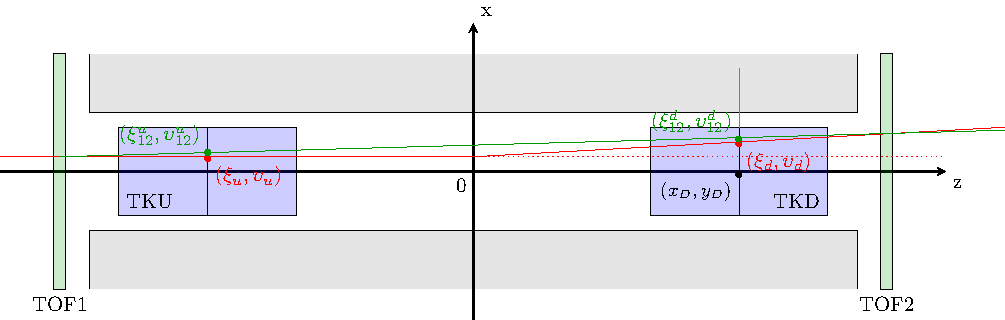
\includegraphics[width=0.95\textwidth]{alignment.pdf}
	\end{center}
	\caption{
		True path of a single particle track (red) and its path as reconstructed from the time-of-flight system (green). The position of the track at the tracker centres is represented by markers.
	}
	\label{fig:align_bl}
\end{figure}

Each TOF provides a single space point in the global coordinate system. This position is assumed to be the true position with a large uncertainty due to the limited granularity of the detector.
Trackers sample the particle track in five different stations and this allows for the reconstruction of a straight track without any assumption made on the prior position of the tracker.
In global coordinates, on average, the track reconstructed between TOF1 and TOF2 should agree with the track reconstructed in either tracker, i.e. the mean residuals should be zero. Applying this reasoning to the unknown offset and angles yields to a system of equations for the four unknown constants~\cite{2018arXiv1805.06623T}.
The measurement of four residual distributions per tracker yields the alignment constants.
The main source of bias is the scattering in the material between TOF1 and TOF2. If the beam is not perfectly centred, particles preferentially scrape out on one side of the magnet bore, anisotropically curbing a specific tail of the residual distribution. To nullify this effect, a fiducial cut is applied to the upstream sample. Only particles that are expected to be contained in the downstream tracker are included in the analysis.

Data is recorded with the superconducting magnetic channel of the experiment turned off, i.e. with tracks going in a straight line from TOF1 to the beam dump. High momentum beams are used in order to reduce the RMS scattering angle and maximise transmission.  
Each data set was processed independently with the algorithm. Figure~\ref{fig:runtorun} compiles the alignment parameters measured for each run during a specific ISIS user cycle. The measurements are in good agreement with one another and show no significant discrepancy: an agreement between the independent fits guarantees an unbiased measurement of the alignment constants. The constant fit $\chi^2/\text{ndf}$ is close to unity for each fit, which indicates that there are no significant additional source of uncertainty. The optimal parameters are summarised in table\,\ref{tab:201701_constants}. 

\begin{table}[ht!]
	\centering
		\begin{tabular}{l|c|c|c|c}
			& x [mm] & y [mm] & $\alpha$ [mrad] & $\beta$ [mrad] \\
			\hline
			TKU & $-0.032\pm0.094$ & $-1.538\pm0.095$ & $ 3.382\pm0.030$ & $0.412\pm0.029$ \\
			TKD & $-2.958\pm0.095$ & $ 2.921\pm0.096$ & $-0.036\pm0.030$ & $1.333\pm0.030$
		\end{tabular}
	\caption{Summary table of the optimal alignment constants measured in the high-momentum straight-track data acquired during the 2017/01 ISIS user cycle.}
	\label{tab:201701_constants}
\end{table}

\begin{figure} [!htb]
	\centering
	\begin{minipage}[b]{.49\textwidth}
		\centering
		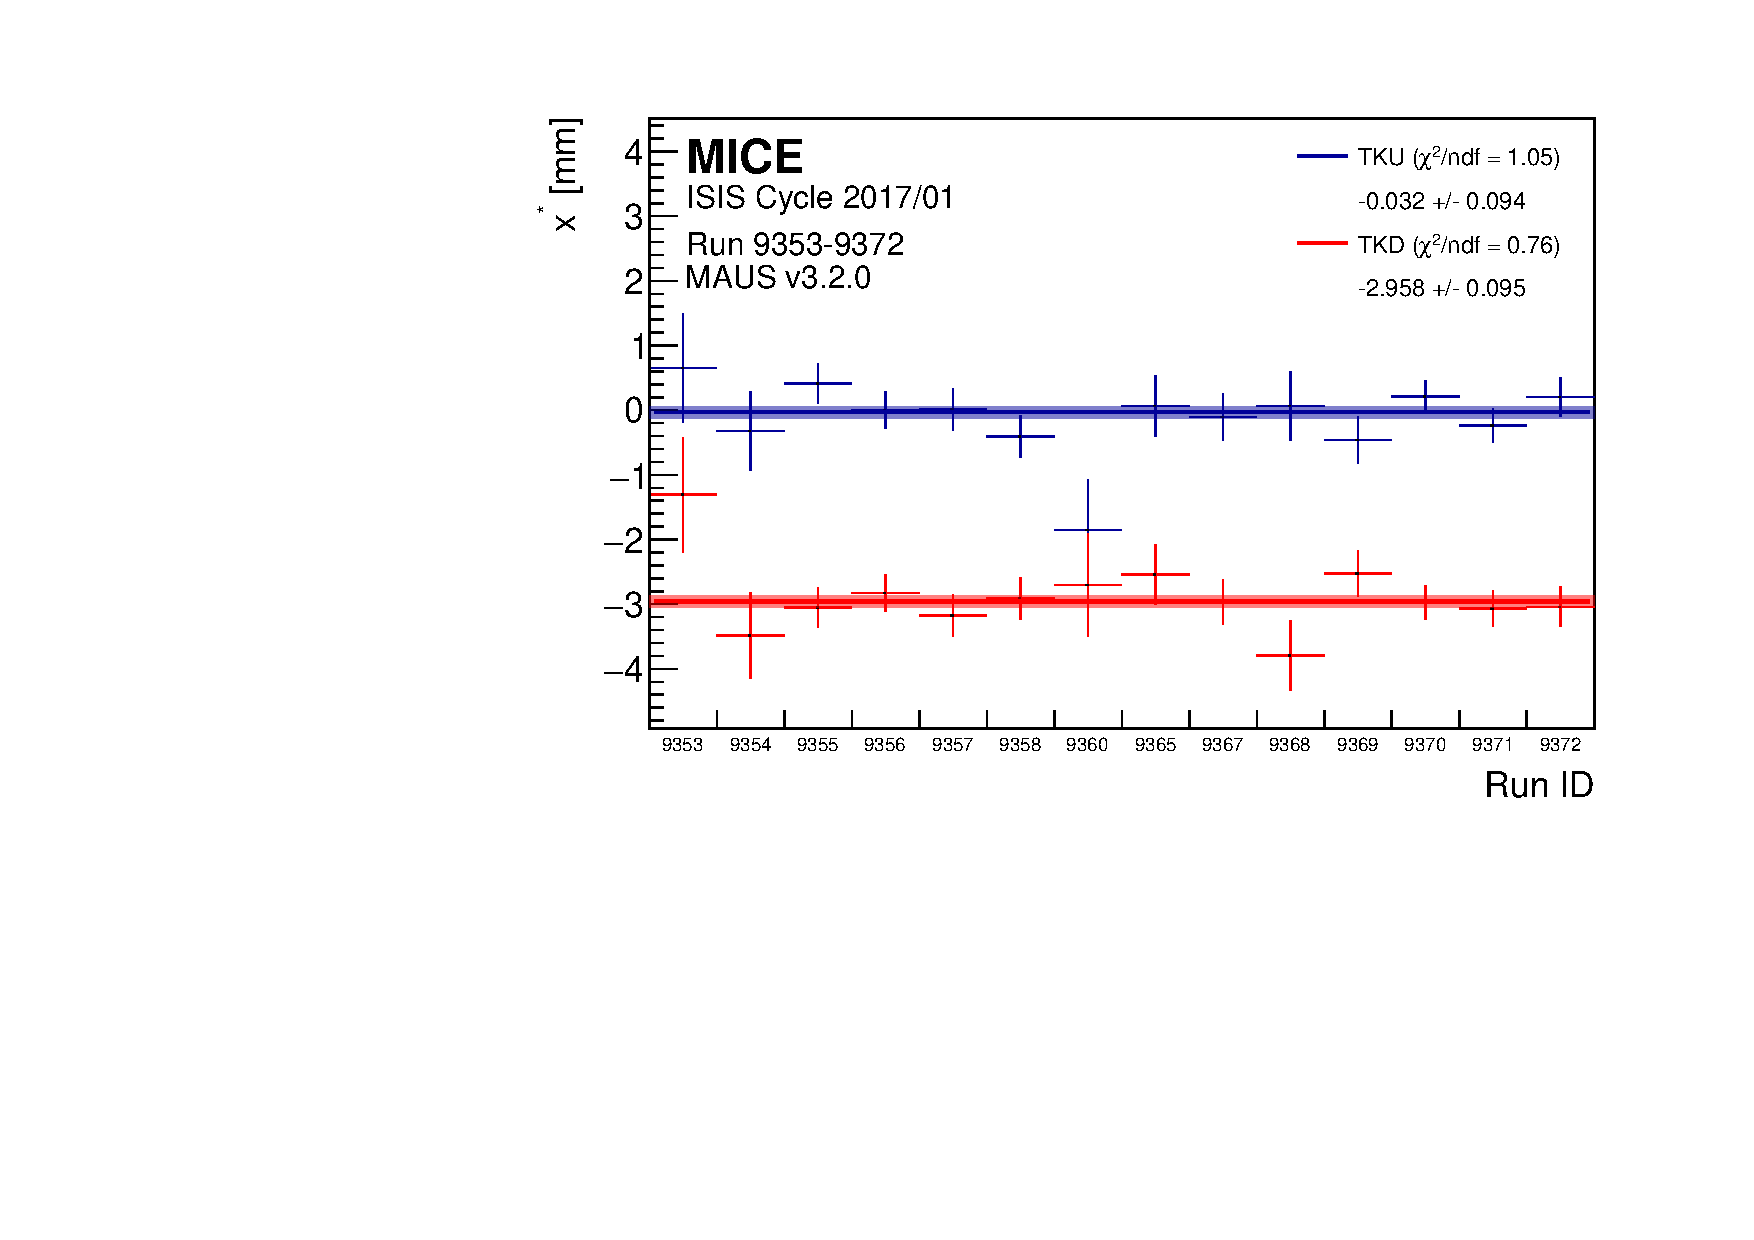
\includegraphics[width=\textwidth]{data_final/x_bestfit.pdf}
	\end{minipage}
	\hfill
	\begin{minipage}[b]{.49\textwidth}
		\centering
		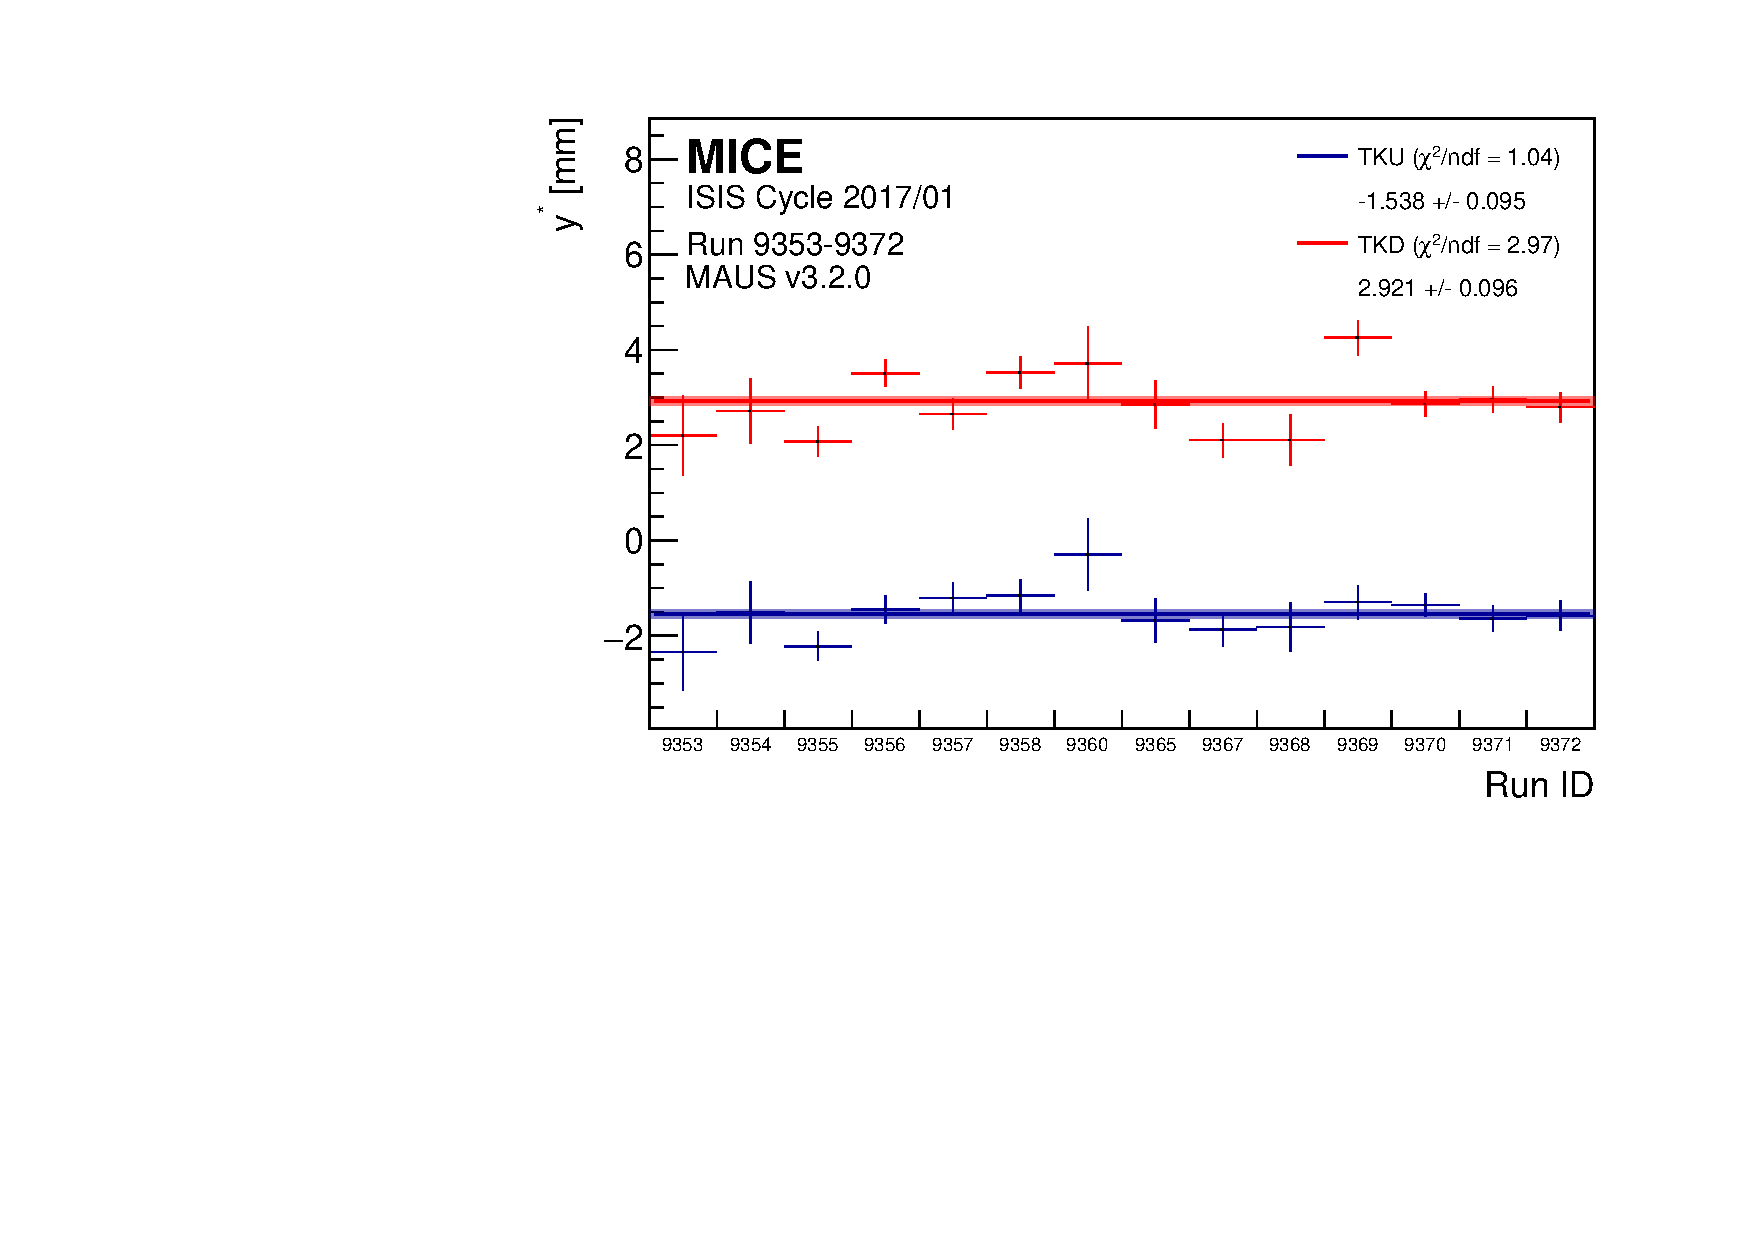
\includegraphics[width=\textwidth]{data_final/y_bestfit.pdf}
	\end{minipage}
	
	\begin{minipage}[b]{.49\textwidth}
		\centering
		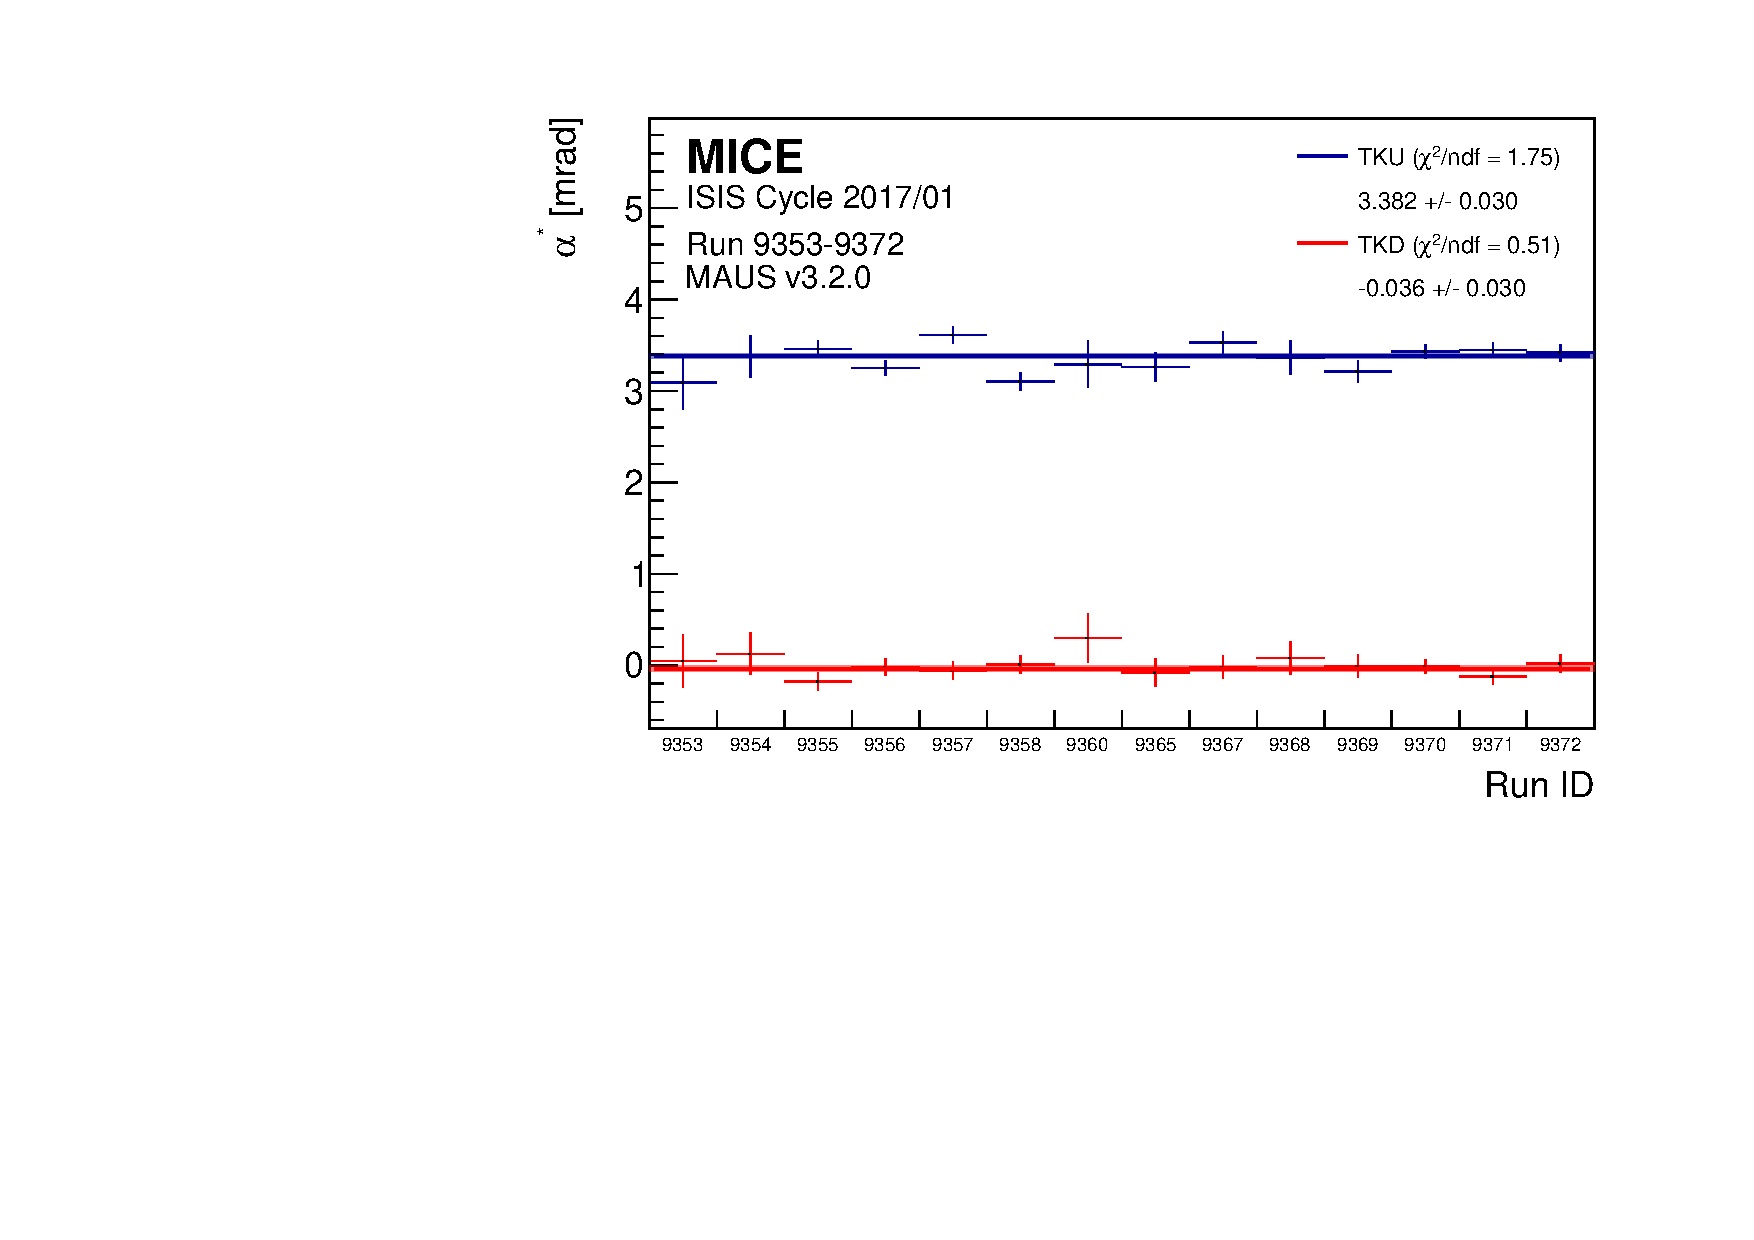
\includegraphics[width=\textwidth]{data_final/alpha_bestfit.pdf}
	\end{minipage}
	\hfill
	\begin{minipage}[b]{.49\textwidth}
		\centering
		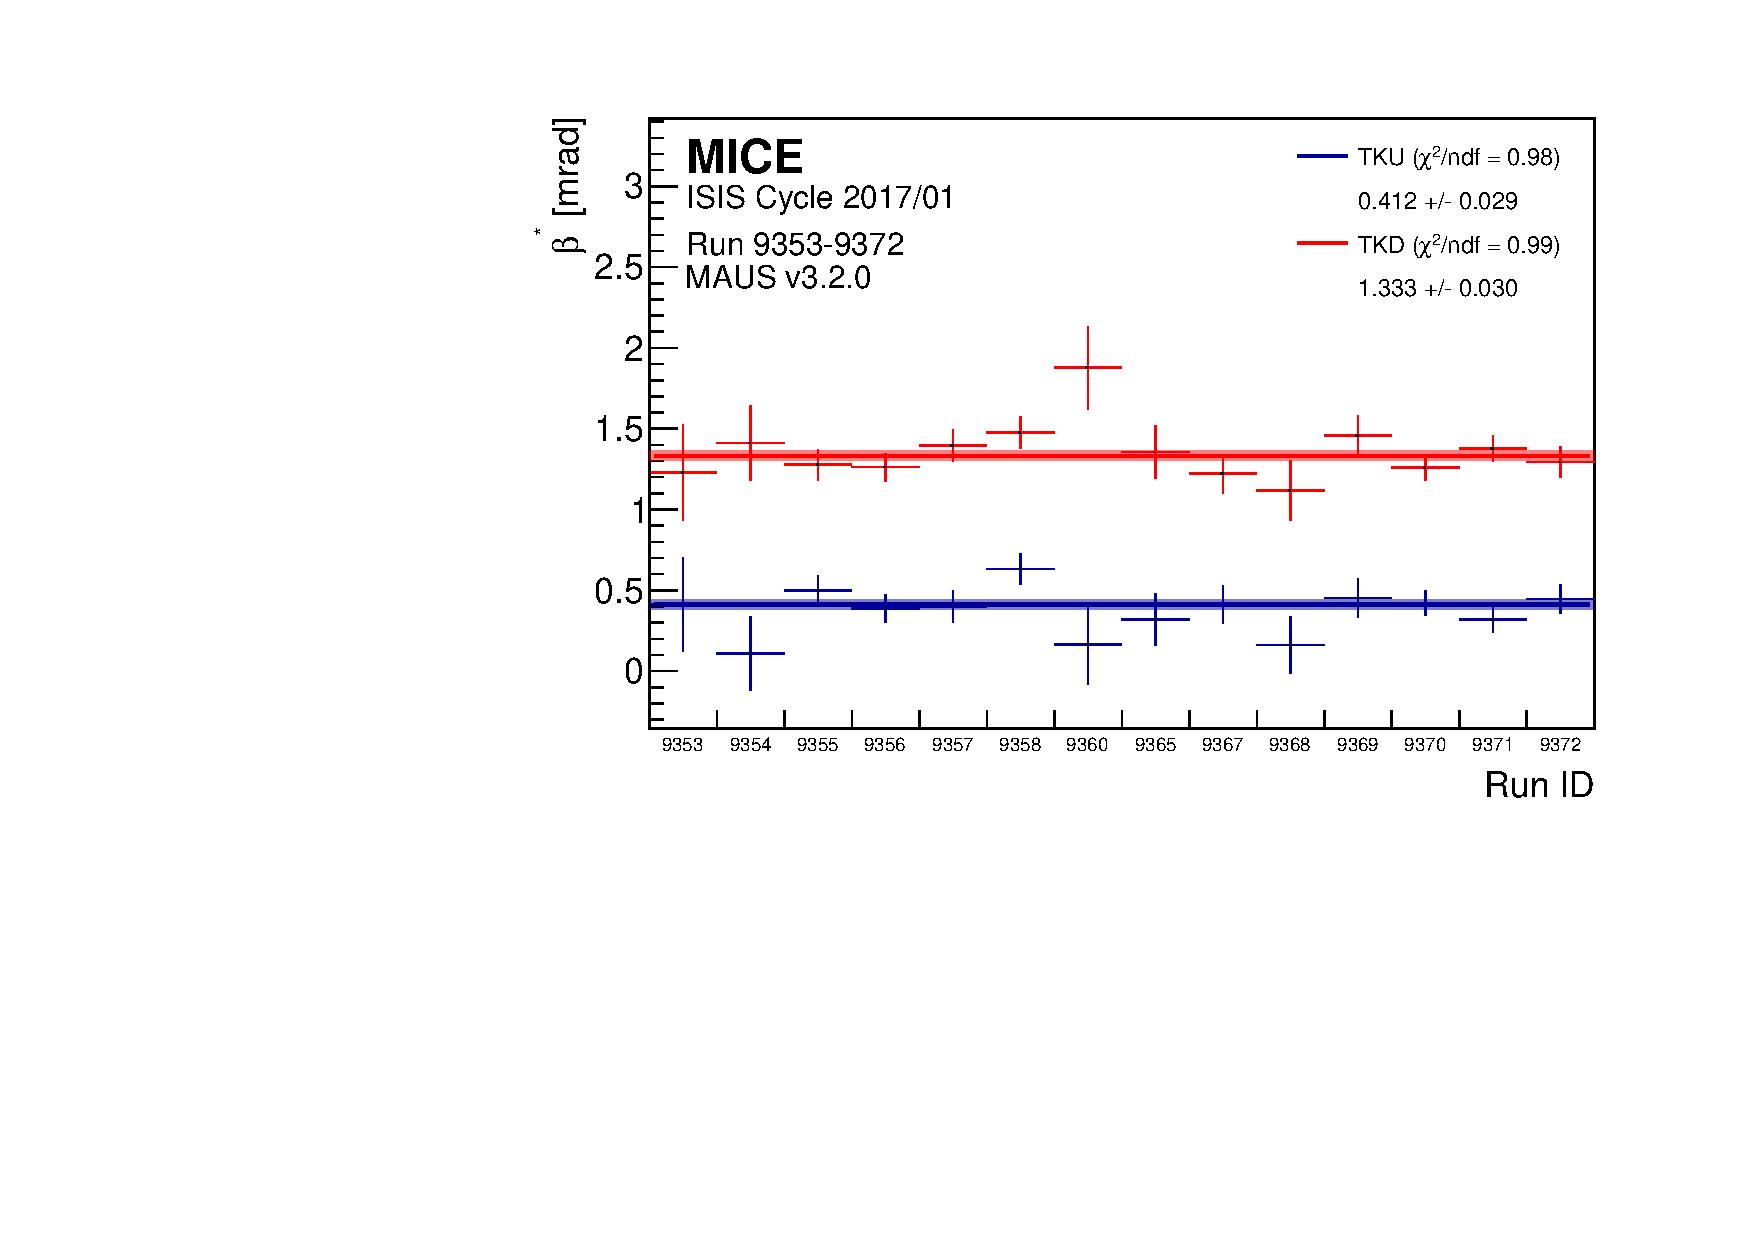
\includegraphics[width=\textwidth]{data_final/beta_bestfit.pdf}
	\end{minipage}
	\caption{Consistency of the alignment algorithm across runs acquired during the 2017/01 ISIS user cycle.}
	\label{fig:runtorun}
\end{figure}
